\section{Marginalisation studies}
\label{app:margstudies}

The increase in sensitivity to \deltacp provided by a doubling of FHC statistics in Run 1-8 relative to Run 1-7c has made sampling of the tails of oscillation parameters (particularly \ssqthonethree) more significant for 1D fits. In previous analyses all fits were performed with 10K marginalisation toys, but in the present analysis this is no longer sufficient to ensure that fits return consistent results for independent sets of marginalisation toys. One can see the nature of the problem in \cref{fig:marginalisation_study_10k}, in which five independent sets of 10K marginalisation toys were fitted under the Asimov A oscillation parameter hypothesis without the reactor constraint; a large spread in $\Delta\chi^2$ contours is evident.

\begin{figure*}
	\center
	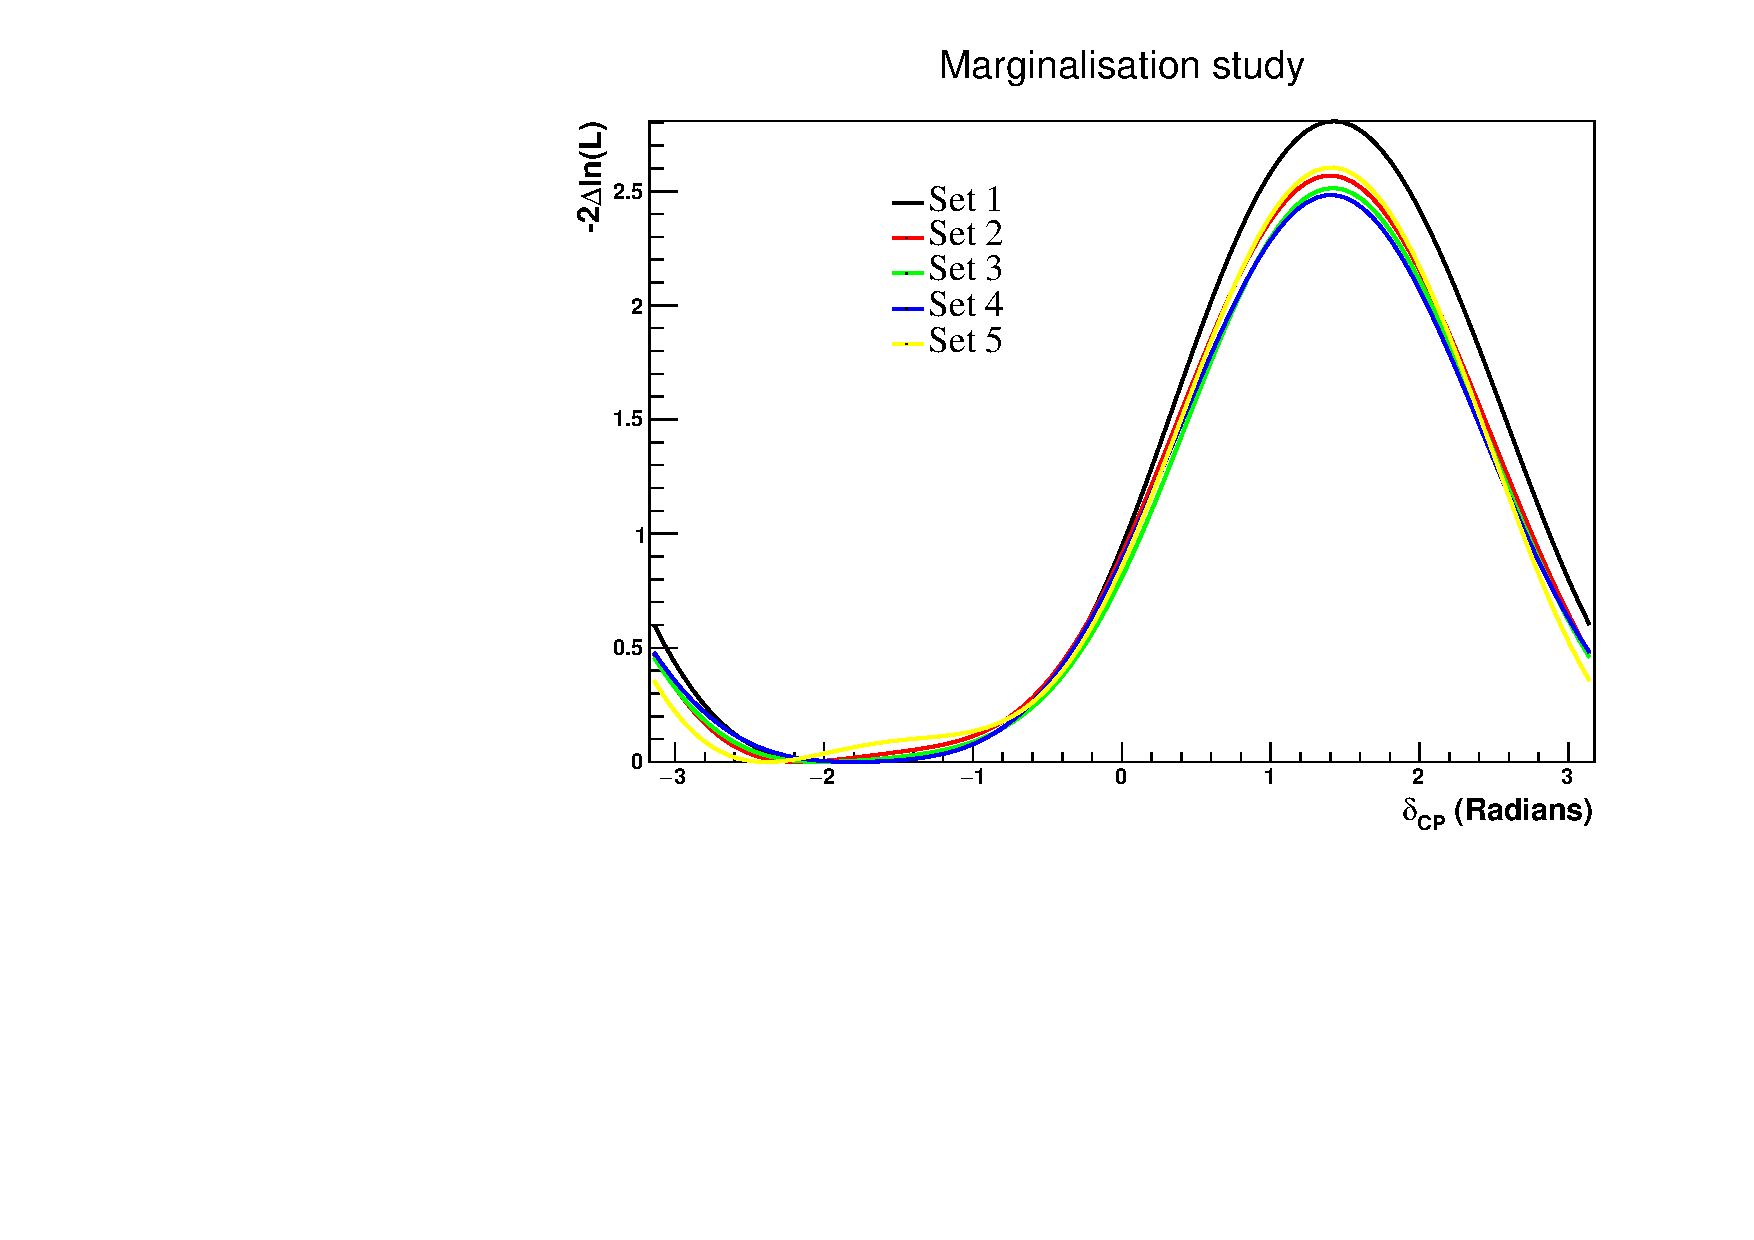
\includegraphics[width=0.75\textwidth]{studies/marginalisation/10k}
	\caption{Asimov A \deltacp normal hierarchy contours without reactor constraint for independent sets of 10K marginalisation toys}
	\label{fig:marginalisation_study_10k}
\end{figure*}

To determine a sufficient number of marginalisation toys to use checks of fit stability were carried out for different numbers of marginalisation toys. \Crefrange{fig:marginalisation_study_40k}{fig:marginalisation_study_80k} show the $\Delta\chi^2$ contours for the case of 40K and 80K marginalisation toys respectively. These studies indicate that good agreement among fits is achieved for 80K marginalisation toys 40k toys was found to be sufficient in the with reactor case due to the smaller marginalisation range for \ssqthonethree).

\begin{figure*}
	\center
	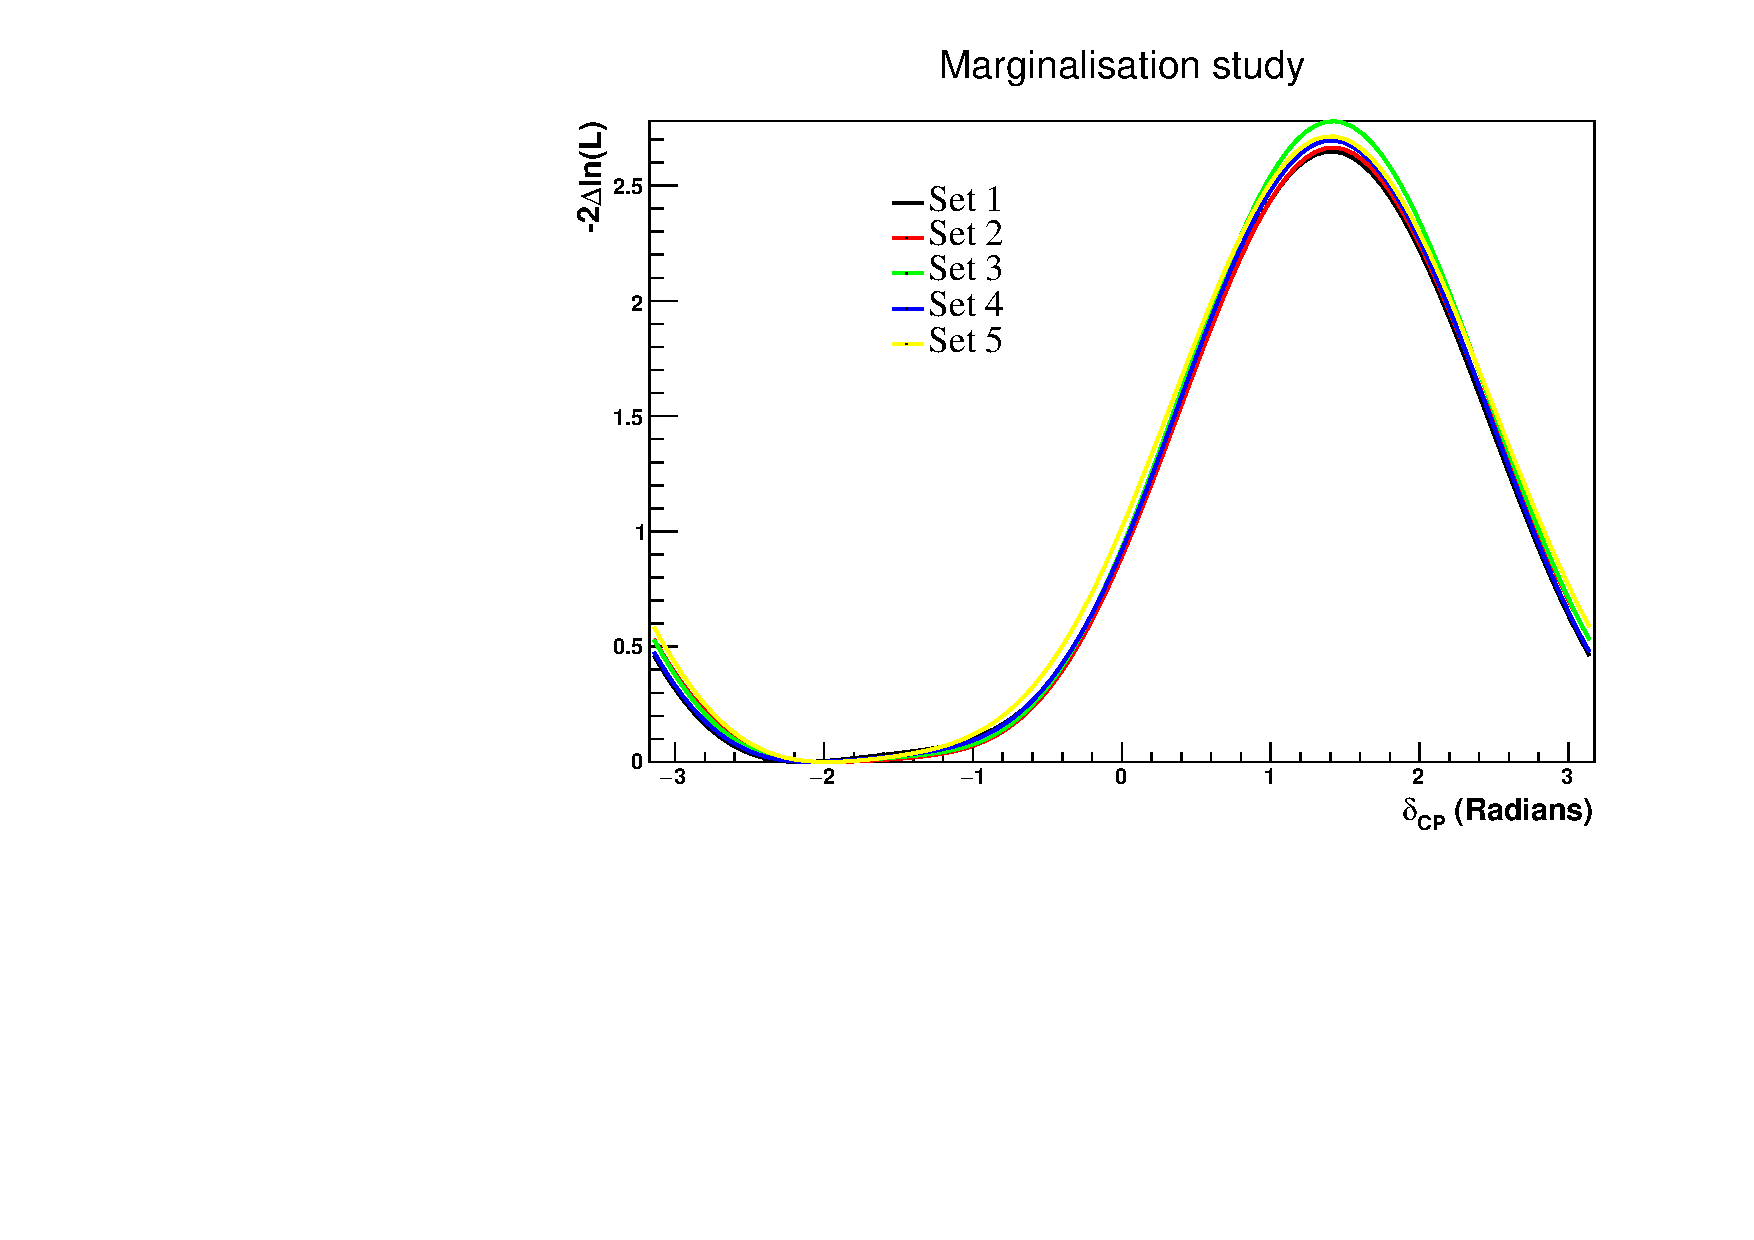
\includegraphics[width=0.75\textwidth]{studies/marginalisation/40k}
	\caption{Asimov A \deltacp normal hierarchy contours without reactor constraint for independent sets of 40K marginalisation toys}
	\label{fig:marginalisation_study_40k}
\end{figure*}

\begin{figure*}
	\center
	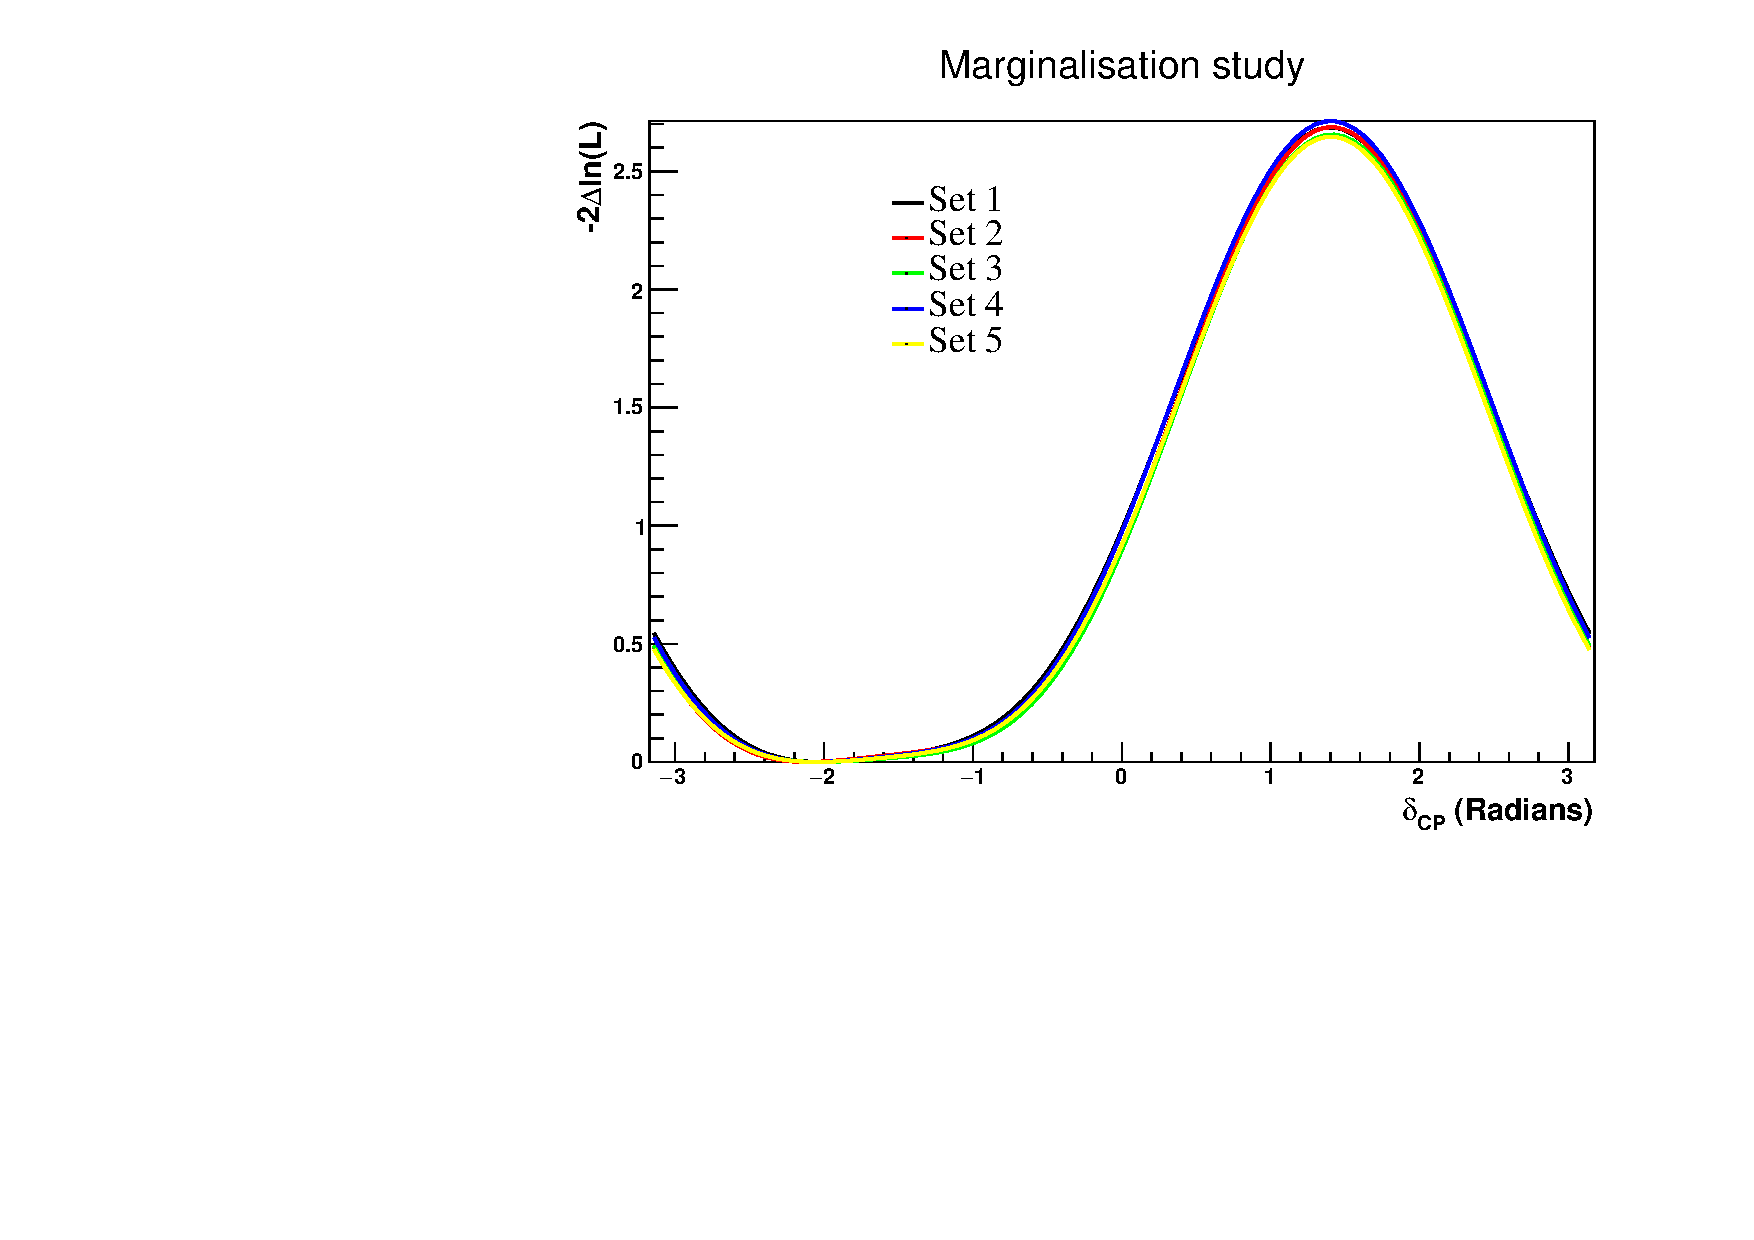
\includegraphics[width=0.75\textwidth]{studies/marginalisation/80k}
	\caption{Asimov A \deltacp normal hierarchy contours without reactor constraint for independent sets of 80K marginalisation toys}
	\label{fig:marginalisation_study_80k}
\end{figure*}

Further to the Asimov-based marginalisation studies, the stronger constraint seen in the data fits prompted a check of the data fit stability. \Crefrange{fig:marginalisation_data_study_nh}{fig:marginalisation_data_study_nh} show the result of fitting \deltacp with the reactor constraint for both normal and inverted hierarchy. Variations of $\Delta\chi^2\sim 1$ are evident around the maximum in the region of $\delta_{CP}\sim\pi/2$, but that good stability is maintained in the preferred region and at the values of $\delta_{CP} = 0$ and $\pi$.

\begin{figure*}
	\center
	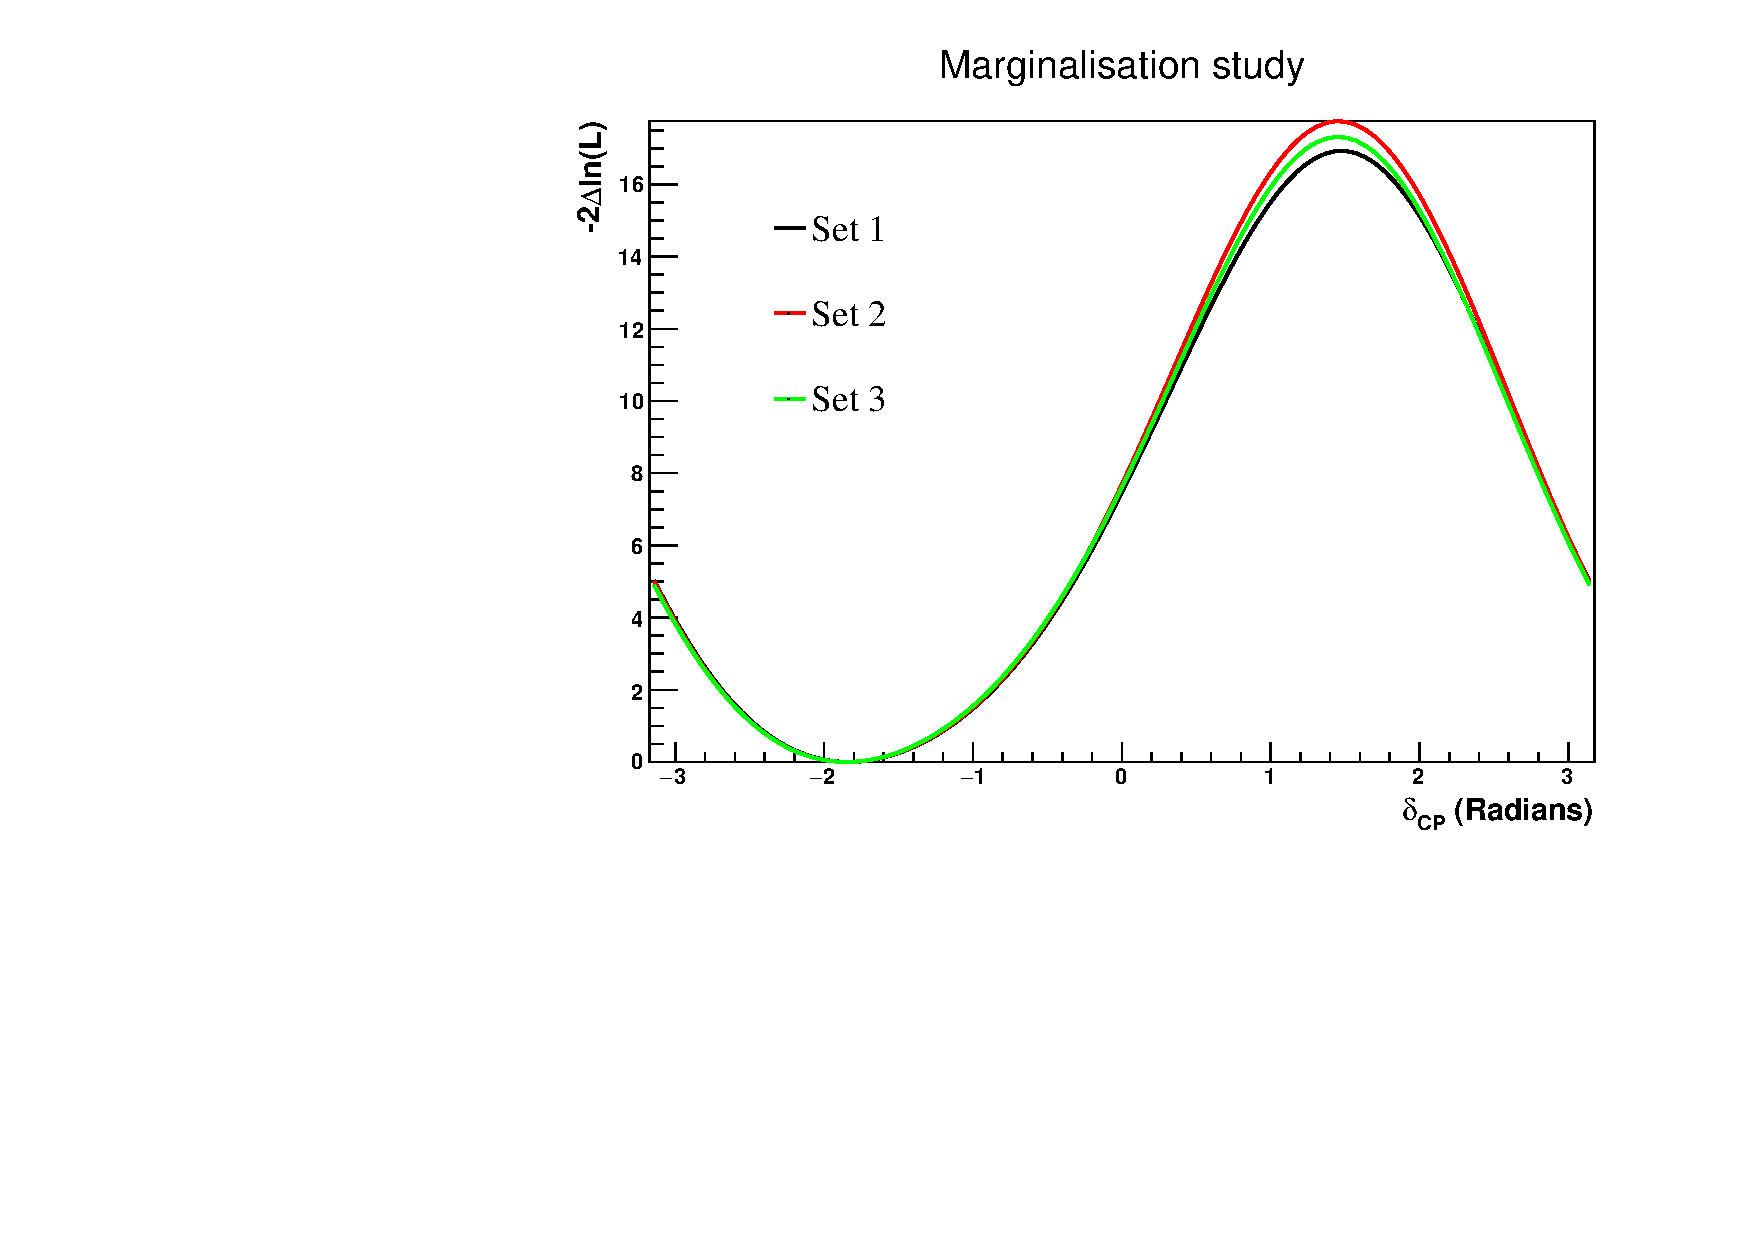
\includegraphics[width=0.75\textwidth]{studies/marginalisation/data_study_nh}
	\caption{Data fit of \deltacp normal hierarchy contours with reactor constraint for independent sets of 40K marginalisation toys}
	\label{fig:marginalisation_data_study_nh}
\end{figure*}

\begin{figure*}
	\center
	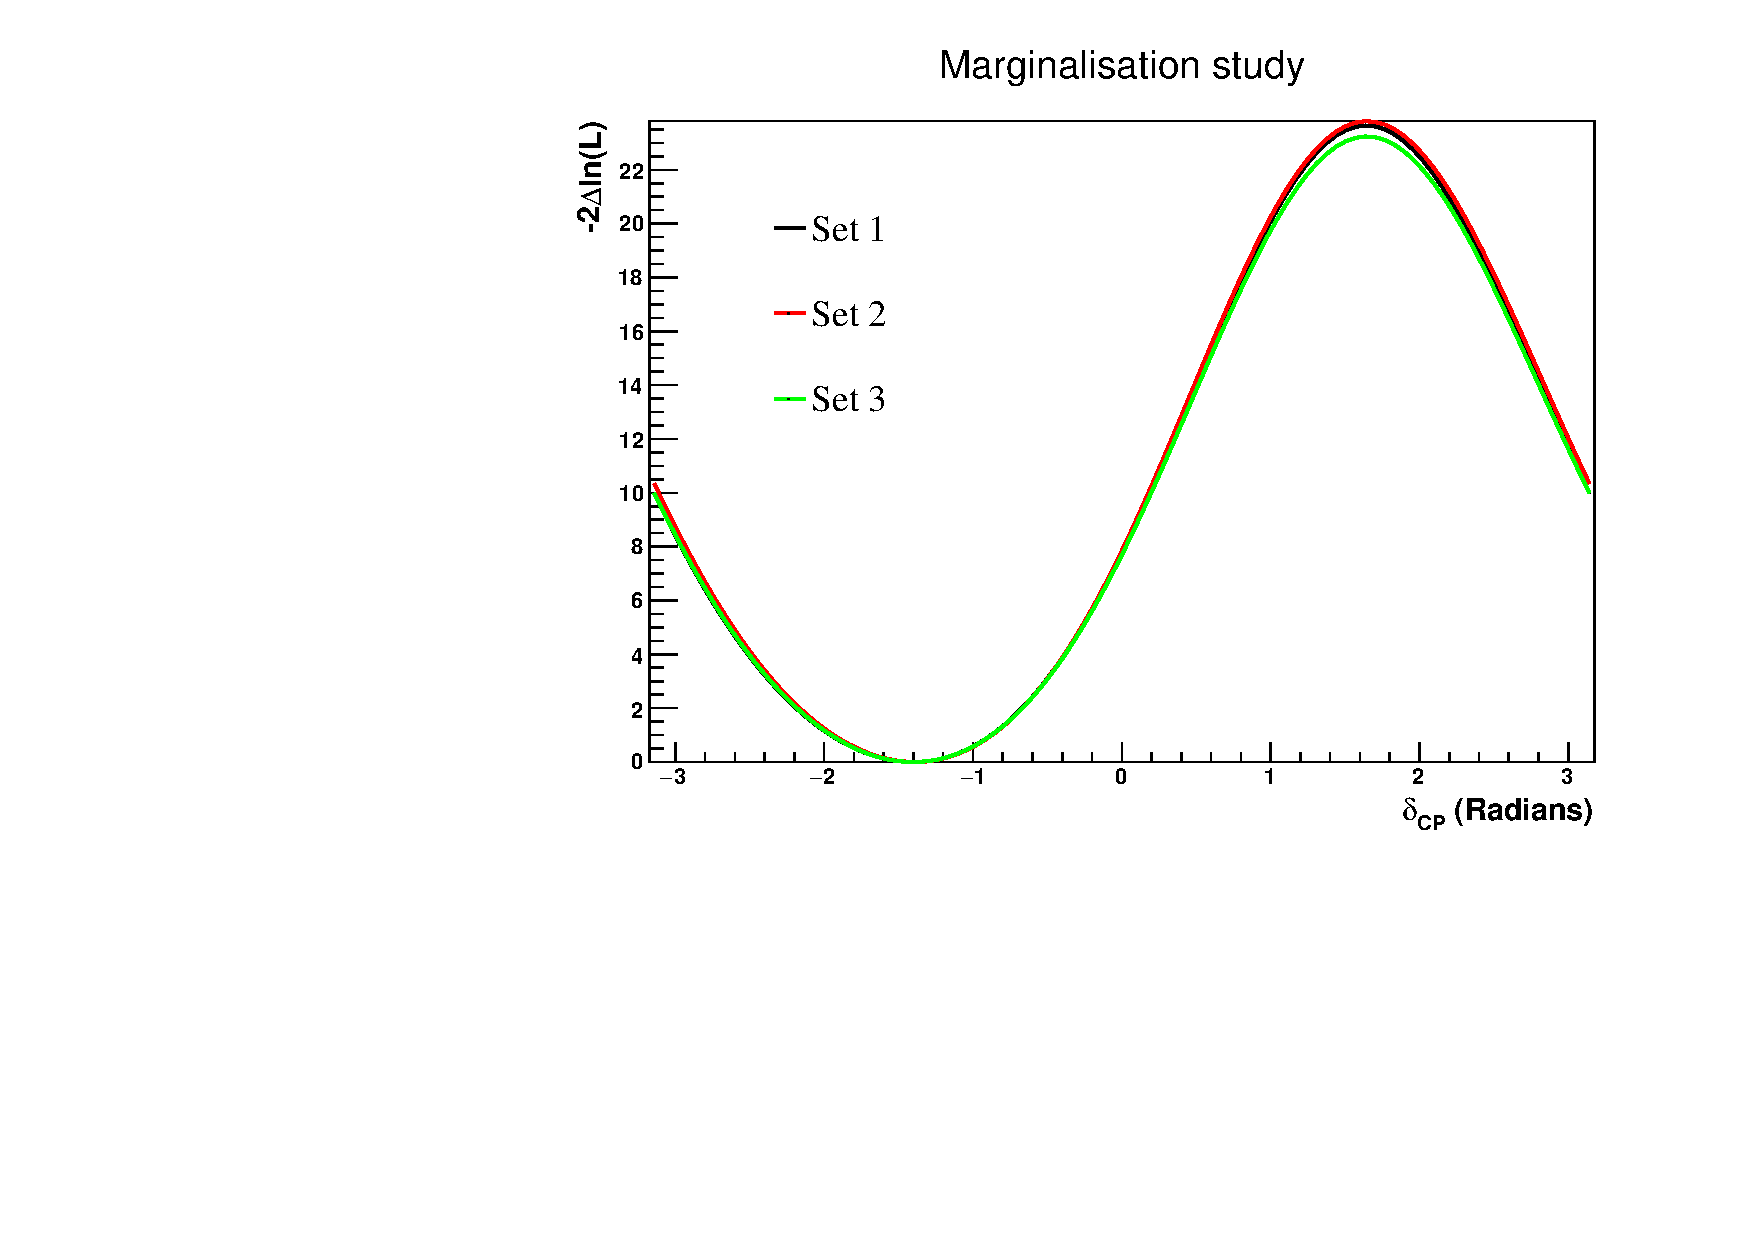
\includegraphics[width=0.75\textwidth]{studies/marginalisation/data_study_ih}
	\caption{Data fit of \deltacp inverted hierarchy contours with reactor constraint for independent sets of 40K marginalisation toys}
	\label{fig:marginalisation_data_study_ih}
\end{figure*}
\clearpage